\documentclass[master, english]{ihethesis}

\usepackage[nottoc,chapter]{tocbibind}					% Add bibliography/index/contents to Table of Contents
\usepackage{microtype}									% Subliminal refinements towards typographical perfection
\usepackage{booktabs}									% The pack­age en­hances the qual­ity of ta­bles in LaTeX
\usepackage{tabularx}									% Tabulars with adjustable-width columns
\usepackage{floatrow}									% Modifying the layout of floats
\floatsetup[table]{capposition=top}
\floatsetup[figure]{font=footnotesize}
\usepackage{romannum}									% Generate roman numerals instead of arabic digits				
\usepackage{amsmath}									% AMS mathematical facilities for LaTeX
\usepackage{amssymb}									% TeX fonts from the American Mathematical Society

\usepackage[product-units = single, multi-part-units = brackets, detect-all, load-configurations=abbreviations, range-units = repeat, separate-uncertainty = false, per-mode=symbol]{siunitx} 			% Correct use of SI units
%\newcommand{\SIp}[2]{\SI[product-units = power]{#1}{#2}} % p for power (chip size...)
%\newcommand{\SIrangem}[2]{\SIrange[range-phrase = --]{#1}{#2}}
%\newcommand{\SIrangecp}[2]{\SIrange[range-phrase = --, range-units = brackets, output-complex-root = j, complex-root-position = before-number]{#1}{#2}}
%\sisetup{separate-uncertainty}%
\newcommand{\SIr}{\SIrange[range-units = single]}

\usepackage{epstopdf}									% Convert EPS to 'encapsulated' PDF using Ghostscript
\usepackage[small]{caption}								% Customising captions in floating environments
%\usepackage{subcaption}
%\usepackage{transparent}
\usepackage[percent]{overpic}							% Combine LaTeX commands over included graphics
\usepackage[title,header]{appendix}						% Extra control of appendices
%\renewcommand{\appendixpagename}{Anhang}
%\usepackage[usenames,dvipsnames,svgnames,table]{xcolor}
\usepackage{color}										% Colour control for LaTeX documents

% Hoehe des Headings anpassen um Fehlermeldung zu unterdrücken, ansonsten folgende zeile wieder löschen:
\setlength{\headheight}{1.5\baselineskip}

\mathchardef\mhyphen="2D
\definecolor{grey}{RGB}{228,228,228}

%\usepackage[pdftex
%            %,colorlinks
%            ,hidelinks %% keine roten Rahmen um Links
%            ,hyperindex
%            ,plainpages=false
%            ,bookmarksopen
%            ,bookmarksnumbered]{hyperref}
%            
%\hypersetup{
%pdftitle={\@title},
%pdfauthor={\@author},
%pdfsubject={\@title},
%%,pdfborder={0 0 0}
%%colorlinks=true,
%%linkcolor=red,          % color of internal links
%%citecolor=black,        % color of links to bibliography
%%filecolor=black,      % color of file links
%%urlcolor=black           % color of external links
%}															

\usepackage[acronym, 
						nonumberlist, 
						toc, 
						nopostdot, 
						style=alttree, 
						nogroupskip]
												{glossaries}
% Nopostdot omits dots at the end of each entry, alttree makes two columns (use \glssetwidest), alternative style=long, nogroupskip no groups by first letter
\setacronymstyle{short-long}
\glssetwidest{$L_{\left(C-package\right)_{eff}}$}% widest name
\renewcommand*{\glsnamefont}[1]{\textmd{#1}} % Define font of entry name
\begin{itemize}
\item firstAkk = fAK
\end{itemize} % Input glossary entries
\makeglossaries
\newcommand{\markup}[1]{\textbf{#1}} % vor \mainpart wird \markup so definiert, dass er nichts mehr macht.


%Abkürzungsverzeichnis
%\usepackage[intoc]{nomencl}
%%\renewcommand{\nomname}{Abkürzungsverzeichnis}
%\setlength{\nomlabelwidth}{.20\hsize}
%\let\ab\nomenclature
%\makenomenclature
\makeindex
%%%%%%%%%%%%%%%%%%%%%%

\makeatletter
\renewcommand\bibsection{
      \chapter*{\bibname\@mkboth{Literaturverzeichnis}{Literaturverzeichnis}}}
\makeatother

%########
\graphicspath{{graphics/},{graphics/snr/},{graphics/simulation/},{graphics/concept/}}
%############################

%#################################################################
% begin document
%#################################################################

\begin{document}

\title{Evaluation, design and realisation of a Riemann Pump for the frequency range of 0..6 GHz for 5G mobile communication}
\author{Markus Wei\ss}
\betreuer{Prof.~Dr. Oliver Ambacher}
\zweitbetreuer{PD~Dr.~techn. R\"udiger~Quay}

\datestart{01.11.2015}					% starting and ending date
\dateend{30.04.2016}

\abstract{\textbf{Agenda}
\begin{enumerate}
	\item literature survey [3 papers + X]
	\item adaption of push-pull concept from Maksimovic
	\item GaN25 \gls{ab: GalliumNitride} parameter simulation [S-parameter,ON/OFF state]
	\item determine load impedance [input of PPA - GaN25]
	\item determine dimension of transistors
	\item tuning schematic parameter for optimal simulation
	\item enhancement/extension of 1-bit push-pull to 3-bit push-pull stage
	\item digital input control voltage
	\item determine eight slopes of the current sources in schematic
	\item Riemanncode generation with MatLab
	\item control schematic with theoretical input [Riemanncode]
\end{enumerate}
\vspace{1cm}
\textbf{Problems}
\begin{enumerate}
	\item frequency dependent load impedance
	\item the absence of accurate current sources makes it very hard to get a defined slope for the switching transistors.
	\item theoretical slope generation very inaccurate
	\item theoretical slope generation via shorted load  (R = 1 Ohm)
	\item $\rightarrow$ slopes ambiguous
	
	\item $\rightarrow$ riemanncode generation not possible                                                                                                                                                                                                                                                                                                                                                                                                                                                                                                                                                                                                                                                                                                                                                                                                                                                                                                                                                                                                                                                                                                                                                                                                                                                                                                                                                                                                                                                          
\end{enumerate}
\vspace{1cm}
\textbf{questions}
\begin{enumerate}
	\item mmW band much higher BW,Datarate,Spectrum - why use the old fashioned frequency bands from DC to 6GHz instead of using a couple of GHz?
	\item trade off between BW and losses
	\item higher frequencies - higher losses (e.g. weather condition, like rain)
	\item 
\end{enumerate}}
		

\maketitle	% generates title page, declaration and abstract page
\pagenumbering{roman}	% pages before TOC
\cleardoublepage
\newpage
\thispagestyle{empty}

%\addcontentsline{toc}{chapter}{\numberline{}Themenblatt}

\tableofcontents

\printglossaries
%\printnomenclature

%\listoffigures
%\listoftables

\cleardoublepage
\setcounter{page}{1}

\pagenumbering{arabic}
\chapter{Preface}
Mobile communication became a major part of our daily life. In our every day life applications such as Instagramm, Whatsapp, facebook and Snapchat  are dealing with very high data transfer rates. The industry also handles a very big amount of data. Real time trading at a stock exchange market is crucial, so the industry tries to reach this with the help of RF mobile communication. The data rate is increasing exponentially up to the year 2020. Todays hardware architectures can not handle this amount of data. In the next generation, the fifth, of mobile communication different concepts are needed to deal with this high data rate. In the next generation new hardware architecture are needed. This new concepts are based on the idea of a full software radio. The concept is basically to bring the digital domain as close as possible to the RF Front-End. Therefore the filter, mixer and computation would be much faster, more accurate and less complex. 


\chapter{Research and Development of 5G mobile communication}
\textit{An optic survey of the state-of-the-art with extensive references.}
State of the art of the next generation of mobile communication. Mobile Congress 2016 in Barcelona, Huawei \& Telekom present a first data link in 73 GHz with a few Gbps.\\
First attempts on a digital to analog converter for the frequency range based on the concept of a charge pump, were designed by french people Veyrac et. al\\
Mark Zuckerberg hold a speech about fifth generation of mobile communication. The goal is to provide and deliver internet to everyone in every country.  
\chapter{Fundamentals of the Riemann Pump}
\label{ch:fundamentals}
%\textit{Presentation of the theoretical basis required for an understanding of your work. Do not begin with Newton's laws or Maxwell's equations: imagine that the reader is a competent engineering professor, but not necessarily in your field of expertise. Do not bother to discuss any theory that you do not employ in later sections.}
For the purpose to place this work into the context of the next generation of mobile communication, the concept of software-defined radio is described.
Implemented in this concept, the function, the benefit and some fundamentals of the Riemann Pump are described. 
A demonstrated system shows the \gls{ab:sdr} concept, which is based on the idea to bring the digital domain as close as possible to the antenna.
The Riemann Pump is an arbitrary waveform generator which is controlled by a digital input signal, making it also a custom \gls{ab:dac}.
The concept of the custom designed \gls{ab:dac} as well as some characteristics are presented.
A concise discussion conclude the presented fundamentals.

% Because the analog output signal should be transmitted via an antenna, it has to be enough output power.
%The number of bits, hence the resolution of the \gls{ab:dac} is less stringent as the digital to analog conversion do not distinguish so much within the digital code.
% A crucial point to increase the performance is the oversampling ratio. 
% As the analog signal could consist with some concurrent signals, linearity is crucial to avoid unwanted distortions.
%All these requirements built in one \gls{ab:dac} is not realistic.
%Therefore, intermediate systems have been developed in which the transmitter signal is built by a DAC at lower frequencies, and then up converted with RFFE mostly composed by a linear mixer with a linear PA.
\section{Basic concept of software-defined radio for 5G mobile communication}
The ultimate software defined radio architecture is shown in Figure \ref{fig:ultimateSDR}.
In this vision the analog received signal is directly converted into the digital domain and afterwards filtered, mixed, demodulated and processed.
The absence of the \gls{ab:rffe} is a dream still to come true \cite{RivetDevalJ.-B.EtAl2010}.

\begin{figure}[ht]
	\centering
  \includegraphics[width=.5\textwidth]{ultimateSDR.pdf}
	\caption{Ultimate Software-defined radio architecture \cite{DevalRivetVeyracEtAl2013}}
	\label{fig:ultimateSDR}
\end{figure}

As Figure \ref{fig:feas_energy} already suggests this is not a realistic option.
The analog components like LNA,filter, mixer have to be implemented separate in the analog domain for the receiving path.
As the transmitter concept is little bit easier

\begin{figure}[htbp]
	% minipage mit (Blind-)Text
	\begin{minipage}{0.49\linewidth} 
	\includegraphics[width=1.1\textwidth]{energy_consumption_sdr.pdf}
	%\caption{Feasibility of Software Radio}
	%\label{energy1} 
	\end{minipage}
	% Auffüllen des Zwischenraums
	\hfill
	% minipage mit Grafik
	\begin{minipage}{0.49\linewidth}
	% \textwidth bezieht sich nun auf die Minipage
	\includegraphics[width=1.1\textwidth]{energy_consumption_sdr2.pdf}
	%\caption{Estimated energy consumption}
	%\label{energy2} 
	\end{minipage}
 \caption{Feasibility (left) and estimation of energy consumption (right) regarding Effective number of Bits and Sample Rate \cite{RivetDevalJ.-B.EtAl2010}}
 \label{fig:feas_energy}
\end{figure}



\section{System design using the Riemann Pump} % PLL and Energy consumption
The focus in this thesis was on the transmitting path of the mentioned system, since the receiving architecture and concepts need a separate investigation.
Further details on the receiving concepts and investigations can be found in \citep{RivetFadhuileDevalEtAl2013}, \cite{RivetDevalD.2008}, \cite{RivetF.2014}, \cite{RivetDevalBegueretJ.-B.2007}.
Focussing on the transmitting path the demand of a \gls{ab:dac} became visible as the digital data must be converted to the analog signal before transmission via the antenna.
As mentioned before high demands are made to the \gls{ab:dac} implemented in a \gls{ab:sdr} concept.\\
One very important requirement is to keep the energy consumption in a moderate range.
If the consumed energy is in the range of several \si{\kilo \watt} it is clear that this is unworkable.
In order to meet \gls{ab:rf} standards the \gls{ab:snr} has to fulfil the limits.
To achieve a moderate \gls{ab:snr} the resolution and the \gls{ab:osr} of the \gls{ab:dac} have to be tuned.
Another crucial aspect is the linearity of the system to avoid unwanted distortions in the propagated signals.
The generated analog output signal, which can consist of a few concurrent signals, has to be amplified for the propagation.\\
The concept of software-defined radio is treated to overcome old problems of mobile communication and hence deal with a fast adapting system which can handle several mobile communication standards at once.
New standards can handled since the system can be changed with an firmware update. 
Therefore every signal within the proposed bandwidth could be processed without changing the hardware, which made it software defined.
The ability to process a spectrum of \gls{ab:dc} to \SI{6}{\giga \hertz} enables it to deal with future mobile communication standards, e.g. IEEE802.11ac (\gls{ab:wlan}) and \gls{ab:lte} already work at \SI{5}{\giga \hertz} and \SI{0.7} ... \SI{2.6}{\giga \hertz}, respectively.\\
To achieve this goal it is essential to bring the digital domain as close as possible to the antenna \cite{RivetDevalBegueretJ.-B.2007}, \cite{DevalRivetVeyracEtAl2013},\cite{RivetDevalJ.-B.EtAl2010}.
The digital domain has a lot of advantages regarding complexity, cost, filtering and processing speed \cite{Grossman2005}.
The structure of digital components is less complex and therefore has less cost.
Digital filtering is more precisely and data processing is more efficient and faster \cite{Chamberlain2015}, \cite{LiRaghunathanJha2009}.\\
% Therefore there is no intermediate step of signal processing which decrease the latency.
%The benefit of this concept is to realize this \gls{ab:dac} as close as possible to the RF front end without an intermediate step of analog signal processing.
% The main drawback of this approach is the energy consumption based on an inefficient ADC/DAC.
%Based on this concept a digital-analog converter is designed to deal with a higher bandwidth than other devices nowadays.
Figure \ref{fig:System} demonstrates the transmitting path of the system design for the concept of \gls{ab:sdr} with the implementation of the Riemann Pump.

\begin{figure}[ht]
	\centering
  \includegraphics{SystemDesign.pdf}
	\caption{Concept of the Software-defined radio}
	\label{fig:System}
\end{figure}

The demonstrated path in Figure \ref{fig:System} is subdivided into a digital and analog part.
The green digital part is responsible for the calculation of the desired signals and the generation of the corresponding digital code.
A theoretical wanted signal in the time domain, consisting of multiple modulated signals, is fed to a \gls{ab:dsp} which computes a digital bit-stream.
The so called Riemann Code controls the input of a custom \gls{ab:dac}, called Riemann Pump, which is the interface between the digital and the analog part.\\
In the red analog domain the desired signal is amplified by the implemented power transistor in the Riemann Pump and then propagated via the antenna.
Optionally a mixer can be connected to mix the desired signal to even higher frequencies of several tenth of \si{\giga \hertz}.\\
Beside the advantages of the concept there are some constraints on the energy consumption as well as on the real time emission.
Energy consumption is increasing linear with the switching frequency and therefore with the signal bandwidth.
Secondly the real time emission is constrained due to the calculation and conversion of the Riemann Code.

\section{Idea of the Riemann Pump}
\label{IdeaRiemannPump}
Demonstrated the implementation of the Riemann Pump in a system design, the concept of the Riemann Pump itself is presented.\\
Basically the inputs are switches and the output is a capacitance.
The output capacitance (\gls{sy:Cout}) can take any value between the positive (\gls{sy:Vdd}) and negative (\gls{sy:Vss}) power supply voltage by controlling the input switches.\\
This concept is implemented in conventional \glspl{ab:pll} and is known as a charge pump, which is the basic principle of the Riemann Pump \cite{DevalRivetVeyracEtAl2013}, \cite{VeyracRivetDevalEtAl2014}, \cite{DevalRivetVeyrac2015}.
 The integration of electrical current (\gls{sy:iout}) at the capacitance (\gls{sy:Cout}) to form the output voltage  (\gls{sy:Vout}), recalls the founder of the integration principle, Bernhard Riemann.
This integration and the concept of the charge pump lead to the name Riemann Pump, first mentioned 2013 in \cite{DevalRivetVeyracEtAl2013}. \\
Figure \ref{fig:ChargePump} shows the basic principle of a charge pump, used for the digital to analog conversion in this thesis.

\begin{figure}[ht]
	\centering
  \includegraphics[width=0.5\textwidth, angle = 270]{ChargePump.pdf}
	\caption{scheme of a charge pump}
	\label{fig:ChargePump}
\end{figure}

Increasing the output voltage lead to close the upper switch, also called high side switch, since it switches to the high power potential.
Synchronously the low side switch opens.
Connecting the high side power supply to the capacitor pumps charges onto it forming a voltage over time.
This effect only takes place if the low side switch synchronously opens.
Otherwise the potential at the capacitor is floating and the charge or discharge process is undefined.
Hence these two switches must be controlled with a differential input signal.
For decreasing the output voltage the low side switch has to be closed, while the high side switch is open, to allow the capacitor to discharge.\\
Corresponding to the described principle the output voltage is calculated with 
\begin{equation}
	V_{out} = \frac{1}{C_{out}}{ \int_0^T \! i_{out}(t) \, \mathrm{d}t}.
\end{equation} %%, \hspace{1cm} T = \frac{2*OSR}{f_{sample}

Since the output voltage, consisting of the desired signals, should be propagated via an antenna, the output capacitance can be interpreted as the input stage of a linear power amplifier. 
This input stage consists of a power transistor, which do have the capacitive input impedance characteristic.
The capacitive input characteristic of the connected power transistor enables the system to work without a separate power amplifier.
Implemented in one component this concept saves area and costs and the amplified signal at the drain can be transmitted via the antenna.

%% 20.04 19:00 Uhr

The Riemann Pump is a digital-to-analog converter based on the concept of a charge pump. A few charge pumps with different sized sources in parallel shows the concept of this fast digital to analog converter. With the ability to control the switches really fast, because of the use of GaN25 technology, which have a high transition frequency, a high bandwidth is reached.

\begin{figure}[ht]
	\centering
  \includegraphics[width=0.5\textwidth, angle = 270]{RP_concept.pdf}
	\caption{Concept of the Riemann Pump with three-bit resolution}
	\label{fig:RiemannPumpConcept}
\end{figure}

 The working principle is to integrate a current into a capacitive load, this integration is based on Riemann Integral, where the name come from. This integration converts the current into a voltage. This output voltage can be applied to the input of a power amp and then to the antenna to propagate it. The current, which charges the capacitive input impedance of the power amp, is controlled by a digital code. A fixed set of slopes, represents the different current sources. A desired signal in the time-domain is generated with MatLab. This signal can consist of many different signals (different carriers and modulation types). This signal is sampled with the given set of slopes. The minimization of the error leads to the Riemann Code. With this Riemann Code (digital) the driver circuit is controlled. This leads to an analog signal formed by the digital input signal. 
 
\begin{figure}[ht]
	\centering
  \includegraphics[width=.75\textwidth]{SlopesAndTable.pdf}
	\caption{slopes and corresponding code of the synthesized signal}
	\label{fig:SlopesAndTable}
\end{figure}

With this information a high speed digital to analog converter is created. In the following the Riemann Integral is shown.

\begin{figure}[ht]
	\centering
  \includegraphics[width=.75\textwidth]{RiemannIntegral.pdf}
	\caption{Integral of the current which pumps charges on to the cap.}
	\label{fig:RiemannIntegral}
\end{figure}
This integral with its slopes as cited in \ref{fig:SlopesAndTable} generates the riemann code which controls the switches of the circuit. This is done by minimizing the error between the theoretical, desired signal and its synthesized one as shown in Fig. \ref{fig:RiemannIntegralError}
 \begin{figure}[ht]
	\centering
  \includegraphics[width=.75\textwidth]{RiemannIntegralError.pdf}
	\caption{Code generation - error minimizing}
	\label{fig:RiemannIntegralError}
\end{figure}
The signal to noise ratio is calculated in equation \ref{eq:SNR_RiemannPumpConversion}. Quantization noise model {reference: analog device}
\begin{equation}
	\text{SNR } [\si{\dB}] = 6.02N + 9.03r - 7.78 + 10\log_{10}(1 - \frac{1}{2}^{N-1} + \frac{1}{2}^{2N})
	\label{eq:SNR_RiemannPumpConversion}
\end{equation}


%Process of the digital to analog conversion:
%\begin{enumerate}
%	\item theoretical signal generation via multiplication of time domain signals
%	\item linear approximation via error estimation to get a sequence of relative slopes
%	\item get binary code of the sequence of slopes
%	\item control switches with this digital code to synthesize the wanted analog signal
%\end{enumerate}

% \textbf{Description of the OSR, Nyquist-Shannon theorem and the SQNR...}
The \gls{ab:osr} is four and hence due to the Nyquist-Shannon theorem, the sampling \gls{sy:freq} is eight times the signal frequency.
This in mind, tuning the sampling frequency will result in tuning the signal frequency.
%\textit{introducing noise due to the conversion}
%\gls{ab:sqnr}
%The deviation of the two signals is lying in the nature of converting digital to analog in form of quantization noise.

\section{Characteristics of Digtial-to-Analog converter}
\label{ch:characteristics}
The characteristics, the performance and figure of merits are compared to classify the Riemann Pump within the conventional digital-to-analog conversion principles.
Performance: Resolution, Maximum sampling rate, dynamic range.
FOM: Gain, SFDR, SNR, settling time.\\
The characteristics of different \gls{ab:dac} is the performance and some figure of merits.
Performance leads to the generation of noise in terms of signal to (quantization) noise ratio.
This \gls{ab:sqnr} gave a good insight to the performance of the corresponding \gls{ab:dac} without to focus on energy consumption nor efficiency.
%\textit{Explain the different SNR (short), display the table to compare them.}


\section{Conclusion of the fundamentals}
In this chapter the implementation of the Riemann Pump in a system design has been presented.
After the description of the classification and application, the concept of the custom \gls{ab:dac} has been described.
After explaining a simple charge pump, a multi bit resolution \gls{ab:dac} have been presented.
The designed custom \gls{ab:dac} has been compared to conventional \gls{ab:dac} concepts.
A concise evaluation states that the Riemann Pump is a great improvement for conventional digital-to-analog conversion concepts.
\chapter{Riemann Pump Circuit design}
\label{ch:design}
\textit{Description of the approach you have taken to solve the scientific or technical problem which you were posed. Outline the design, the methodology and overall structure of your experimental approach}\\ 
The concept of the Riemann Pump as seen in Fig. \ref{fig:RiemannPumpConcept} is realised with the design tool \gls{ab:ads}.
The first step was to design a 
A digitally controlled charge pump with eight different slopes is created, called Riemann Pump. To show that this pump is able to convert a digital signal into an analog one an example code is generated. As a MATLAB algorithm do not exists, which computes the Riemann Code, it is done by hand.
In fact of the high energy consumption, the realized DAC is designed for the integration in a base station. Because it converts a digital bit sequence into an analog rf signal it is implemented in the transmitting path. Based on the idea of a push-pull stage the load impedance of the charge pump is designed first.
\section{Approach and implementation of the Riemann Pump}
One possible approach to design a charge pump as shown in Fig. \ref{fig:RiemannPumpConcept} was with concept of a Push-Pull stage.
The concept of the chosen push-pull stage had the advantage of an integrated driver circuit which allows to switch the high side transistor efficient.
This concept is usually used for power electronics [-> which power electronic, refer to].
The first approach of designing a Riemann Pump was with a concept of a Push-Pull stage. This push-pull stage should charge a capacitive load at the output, which is the same as a normal charge pump. Push-pull stages complementary switch a high- and lowside transistor as in a charge pump. This was one possible approach. Concept of Maksimovic.

\begin{figure}[ht]
	\centering
  \includegraphics[width=1\textwidth, draft]{Active_PullUp3.png}
	\caption{Schematic of a driver circuit with push-pull stage representing one bit of the DAC called Riemann Pump}
	\label{RiemannPump}
\end{figure}

 


\section{Calculation of the load impedance}
For simulation purposes a suitable (appropriate) load impedance was necessary. 
The calculation of the load was based on the idea to drive a (pre-) power amplifier with the synthesized signal.
The advantage would be to synthesize a signal near to the RF- front end e.g. in a base station for mobile communication.
As a \SI{20}{\watt} power amplifier would be taken for the transmitting path of a base station the corresponding gate periphery of a \gls{ab:gan}25 transistor would be \SI{4}{\milli \metre}.
This is a keep it small and simple approach to get a first idea of the concept. Otherwise a more accurate way would be to take a broadband power amplifier as load.
The transistor model with this gate periphery was tuned due to the \gls{ab:mag} to get the complex impedance of the power amplifier.
After the tuning process a S-parameter simulation determined the input impedance of the power amplifier which corresponds to the load impedance of the designed Riemann pump circuit.
This transistor model \gls{ab:hemt} (IAF\_GE\_MSL\_ A204/IAF\_GaN25\_HEMT\_CS\_LS\_SHfull) used in \gls{ab:ads} were modelled at the \gls{ab:iaf}.\\

 The first assumption is that the load is a pre-power amplifier which generate a power of \SI{20}{\watt}. To generate this power, the gate periphery of a GaN25 HEMT has to be \SI{4}{\milli \metre} based on the approximation(- official reference???) \SI[per-mode=fraction]{5}{\watt\per\milli\metre}. To get this gate periphery four transistor in parallel each with 8 finger and \SI{125}{\micro \metre} are designed for the power amplifier. The bias point is determined with the \gls{ab:mag}. Therefore the following load impedance could be determined.
\begin{equation}
Z = R - jX_c
\end{equation}

With the help of the $S_{11}$ parameter plotted in the smith chart Fig. \ref{fig:smith_load_impedance} the load impedance can be determined.
The load impedance got a capacitive reactance.
 The real part of the impedance is roughly $R = \SI{1.89}{\ohm}$, while the imaginary part is capacitive. An important point is the input capacitance is increasing with frequency. While it is normal that the imaginary part of the impedance is increasing with frequency, the input capacitance is not.

 \begin{figure}[ht]
	\centering
  \includegraphics[width=1\textwidth]{S_param_LoadImpedance.pdf}
	\caption{smith chart representing the load impedance}
	\label{fig:smith_load_impedance}
\end{figure}

The load capacitance is calculated through the complex impedance:
\begin{equation}
C = \frac{1}{2 \pi f X_c}
\end{equation}

 \begin{figure}[ht]
	\centering
  \includegraphics[width=0.5\textwidth]{InputCap_LoadImpedance_6GHz.pdf}
	\caption{frequency dependent input capacitance of the load}
	\label{fig:smith_load_impedance_inC}
\end{figure}
\section{Dimension of the used components}
The transistor dimension were... Different for driver circuit and power circuit... resistor to reduce the energy  consumption, for higher efficiency. \\ The
approach of the push-pull stage Maksimovic, Maroldt.\\
Approach of theoretical and synthesized signal -> MatLab generation of Riemanncode, SNR.\\ Stability, driver concept, energy consumption, frequency bandwidth, gain
Schematic design in Advanced Design System 2014. concept, ideas... 
\textbf{length of the bonds, number of bonds, thickness of bonds ask Dirk Meder. A lot of vias - more inductance - voltage drop between layers. short as possible lines, no rechtecke - para caps in the edge. first filter cap to supply pin near the chip. number and cap size determined on experience. }\\
Control voltage of 5 V realization with OPAMPS? Possible to overdrive opamps instead of using broadband ppa. 


\section{Circuit design summary and discussion}
\textit{Drawbacks, problems, challenges.}
Same realisation problems, difficulties: Problem of BANDWIDTH, Vpp of control signal (5V pp for GaN transistors), high side driver, no complementary transistors available in III-V technology, low loss driver, high speed driver, digital control driver, too high energy consumption (stability???)
\textbf{bandwidth limitation}
\textit{The lower bound is determined by the sampling time (inverse of the sampling frequency) and the smallest current achieved with the dimensioned transistors.
 The smallest achievable current times the smallest sampling time (highest sampling frequency) determine the smallest absolute slope achievable. \\
 \textbf{Is every signal possible to create?$\rightarrow$ a rect signal has too steep flanks to create. The signal bandwidth ranges from DC to 6 GHz but what is the amplitude range? Is there a limitation regarding the amplitude?}
\\
The smallest current is determined by the dimension of the transistor, which drives into saturation. 
The smallest saturated current is determined by the push-pull transistor geometry, here: 532 mA.}
\chapter{Circuit simulations for generating various waveform signals}
% Outline the simulation results based on the chosen approach in the previous chapter
% iaf 1220 
To proof the presented concept.
To validate the feasibility of the presented concept, a digital input control code is required.
To synthesize various analog signals the corresponding digital input signal is needed. 
In fact that no MATLAB algorithm exists which computes the Riemann code, it is done by hand. 
In a more enhanced project a MATLAB algorithm would compute this code by minimizing the deviation between a theoretical signal and the synthesized signal.
 The deviation of the two signals is lying in the nature of converting digital to analog in form of quantization noise.
The \gls{ab:dac} designed in this thesis should be able to create various (arbitrary) waveform signals.
The presented Riemann Pump converts a digital input signal into an analog signal.
 To validate the chosen approach a harmonic balance simulation is done with the design tool \gls{ab:ads}.
  With this simulation it is possible to plot the voltage amplitude across the load impedance in the time domain.
   The harmonic balance simulation has the advantage that the whole system is modelled in a steady state mode, so that no transients influences the results.\\
    It is important to note that the simulations are done under ideal conditions and no losses due to conductor impedances are taken into account.
    The modelling of a time domain simulation under real conditions with the exact number, width and length of all bonds and other effects, was(is) beyond the scope of this thesis.\\
    A short stability and energy consumption analysis is done to get an impression of it. 
    The realised circuit is in no way tuned or optimized with respect to these two aspects.
     This two aspects could not be investigated in this thesis due to complexity and time issues, what its meaning is not to belittle.\\
    
The simulation results in which various signals are generated have the same \gls{ab:osr} in common.
The \gls{ab:osr} is four and hence, due to the Nyquist-Shannon theorem, the sampling \gls{sy:freq} is eight times the signal frequency.
This in mind, tuning the sampling frequency will result in tuning the signal frequency. 

\section{Generating various signals with digital input control}
%Time signal simulation with optimized components
Simulation in time domain is required to validate the correct generation of a signal. In fact of the linear approximation of current charging a capacitor this is the only way to verify the output signal. If this signal is confirmed to be as good as wanted, a frequency simulation can show the spurious free dynamic range or whatever which is important to mobile communication. To follow the approach in chapter \ref{ch:design} the components are dimensioned as stated there.\\
 The signals described in this section are generated with the ( \gls{ab:dac} design) Riemann Pump circuit design stated in Chapter \ref{ch:design}. The presented \gls{ab:dac} have a resolution of three bit which generates various signals with an \gls{ab:osr} of four. 
 In this section the components are optimized with respect to the signal integrity. The dimensions of the used components are tuned while simulation to provide the desired output signal.
 
\subsection{sine wave generation in the time domain}
At first a sine wave is generated since this is the most powerful signal form.
Hence a sine wave exists any other signal can be generated representing the sum of sine waves.
To validate the feasibility of the presented concept, a digital input control code is required.
To get this code an approximation by hand is done since no algorithm exists which can compute this.\\
Figure \ref{fig:SineWaveCodeGeneration} presents a by hand approximated sine wave.
This approximation is done with the help of eight different slopes which represents the three bit resolution of the \gls{ab:dac}. The sequence of slopes referred to $i_0$ values is \textit{+7 +3 -3 -7 -7 -3 +3 +7} which represents the following Riemann code:  000 010 101 111 111 101 010 000.
 
 \begin{figure}[htb!]
   \centering
   \includegraphics[width=0.75\textwidth]{RCgeneration_SineWave_byHand.pdf} %width=1
   \caption{Riemanncode generation for a sine wave by hand}
   \label{fig:SineWaveCodeGeneration}
\end{figure}

This generated Riemann code was used to synthesize some sine waves in the frequency range between \gls{ab:dc} and \SI{6}{\GHz}.

\begin{figure}[htb!]
   \centering
   \includegraphics[width=0.75\textwidth]{Vout_sine_sampling_1GHz_1period.pdf}
   \caption{Synthesized signals}
   \label{fig:SynthesizedSignalWithStatedRiemanncode}
\end{figure}


\begin{figure}[htb!]
   \centering
   \includegraphics[width=0.75\textwidth]{Vout_sine_sampling_2GHz_1period.pdf}
   \caption{Synthesized signals}
   \label{fig:SynthesizedSignalWithStatedRiemanncode}
\end{figure}

%
%\begin{figure}
%\centering
%\begin{minipage}{.5\textwidth}
%  \centering
%  \includegraphics[width=1\linewidth]{Vout_sine_sampling_1GHz_1period.pdf}
%%  \captionof{figure}{A figure}
%  \label{fig:test1}
%\end{minipage}%
%\begin{minipage}{.5\textwidth}
%  \centering
%  \includegraphics[width=1\linewidth]{Vout_sine_sampling_2GHz_1period.pdf}
%%  \captionof{figure}{Another figure}
%  \label{fig:test2}
%  \caption{Synthesized signal at \gls{sy:freq}= 1 GHz and 2 GHz with stated Riemann code}
%\end{minipage}
%\end{figure}
%















The time domain simulation of the output voltage in the Riemann Pump circuit exhibits the desired behaviour. 
As seen in Figure \ref{fig:SineWaveSynthVsTheoretical} a sine wave signal can be precisely synthesized. 
The sine wave is expressed as 
\begin{equation}
	v(t)= \widehat{v} \cdot sin( 2  \pi  f \cdot  t + \phi),
\end{equation}
with this parameters: $\widehat{v} = \SI{7.5}{\volt}$, $f = \SI{1}{\giga \hertz}$, $\phi = \pi / 4$.

\begin{figure}[htb!]
   \centering
   \includegraphics[width=0.75\textwidth]{Vout_SynthVsTheo.pdf}
   \caption{Synthesized sine wave with the theoretical sine wave}
   \label{fig:SineWaveSynthVsTheoretical}
\end{figure}

Although the fit seems to be very good, two distortions are visible. 

The deviation of the synthesized signal (black) from the desired one (red) is highlighted in Figure \ref{fig:SineCompare}.
Here the theoretical signal is presented in contrast to the synthesized one with their spectra.
% versus the synthesized signal is presented with their corresponding spectrum
The spectrum (Fourier transformation) demonstrates how accurate the signal is synthesized compared to the desired sine wave.\\
On the top left side the theoretical sine wave is plotted in red. Underneath of it the spectrum states a frequency portion for the direct component at \SI{0} {\GHz} and a fundamental frequency portion at \SI{1}{\GHz}.
This Fourier transformation represents the theoretic frequency portions of a clear sine wave. 
In comparison to this it seems that the synthesized signal on the top right side be a good approximation.
The spectrum on the bottom right side exhibits some distortion induced from the quantization process. 
Beside the direct component and the fundamental frequency component there are some other frequency portions which do not occur in the optimal sine wave spectrum.
The bottom right plot of Figure \ref{fig:SineCompare} shows that the distortion is maximal \SI{1}{\volt} in amplitude at a the third harmonic. The 2nd to 10th harmonic are at most a half of a volt.\\
\textit{The accuracy is very good. This can be verified by the signal to noise ratio -> explain, state the SNR}

\begin{figure}[htb!]
	\centering
  \includegraphics[width=1\textwidth]{SineCompare.pdf}
	\caption{Comparison between a theoretical and a synthesized sine wave with their spectrum}
	\label{fig:SineCompare}
\end{figure}

To address already some limitations (of this approach) which occurred during the simulation Figure \ref{fig:7SignalsSameSlopeInOnePlot} shows seven signals synthesized with the same digital Riemann code but different sampling rates.
The signals amplitude is plotted over the radian, representing two periods of the signal.
The plot over the radian makes it easier to compare the signals while they have different frequencies and hence periods.\\
The shapes of the signals with frequencies between \SI{2}{\GHz} and \SI{6}{\GHz} all nicely fit to the expected synthesized sine wave shape. Due to the different periods of sampling time the amplitude of each signal differs, hence the output capacitor is charged for different times.\\
The black and the blue signal with signal frequency \SI{1}{\GHz} and  \SI{500}{\MHz} respectively differ from the expected shape of a sine wave. While the black signal could represent a sine wave with a DC offset of 7.5Vdc and an amplitude of 7.5V the blue signal already shapes like a rectified sine signal. The blue signal which should represent a sine wave with a signal frequency of \SI{500}{\MHz} is clipped and hence shows the behaviour of a rectangular signal. This undesired behaviour is induced from a fully charged output capacitance. \\
The maximum amplitude for the capacitor is the supply voltage of \SI{15}{\volt}. If this maximum is reached, the signal wave form is clipped right there.


%For the baseband frequency of \SI{500}{\MHz} the sampling frequency is eight times baseband frequency due to \gls{ab:osr} and Nyquist-Shannon theorem.
%A sampling frequency of \SI{4} {\GHz} means a sampling time of \SI{250}{\pico \second}, hence the output capacitance is \SI{20}{\pico \farad} it is charged with  .


\begin{figure}[htb!]
   \centering
   \includegraphics[width=0.75\textwidth]{Vout_sine_7signals_inOne_3bit_osr4.pdf}
   \caption{Signals synthesized with Riemann code introduced with Figure \ref{fig:SineWaveCodeGeneration}}
   \label{fig:7SignalsSameSlopeInOnePlot}
\end{figure}

\subsection{rectified sine wave generation in the time domain}
Based on the same optical approximation of the signal in Figure \ref{fig:SineWaveCodeGeneration} the riemanncode for the half sine is generated. The Riemanncode for the half sine is: 000 010 101 111 000 010 101 111
\subsection{triangular wave generation in the time domain}
This is a triangular wave.


\section{Stability analysis of the realised circuit}
The stability analysis is important to ensure that the circuit under test do not oscillate. 
 To check this, the complex impedance at specific points in the circuit is measured.
 If the real part of the impedance is positive for the whole frequency range of the simulation, it indicates in an easy way that the circuit does not oscillate.
This simulation is done within the ADS tool. 

\section{Energy consumption analysis of the realised circuit}
Due to the idea to use the presented topic for mobile communication it could be implemented in mobile devices, although this thesis only handles the device for the basestation. If it could be used in a mobile device the energy consumption is critical.\\
The energy consumption of the designed circuit in chapter \ref{ch:design} is simulated with \gls{ab:ads}.\\
 For the chips used for the demonstrator refer to the work of Stephan Maroldt who states, that the power consumption is:  divided into static and dynamic ones. The switching losses are greater than the static ones.
The losses are divided into dynamic losses of the switches and static losses.
% switch voltage for on/off state, switch time, static losses and dynamic losses.

\section{Proof of concept simulation with existing components}
This simulation is based on the measurements and the design of various chips from Stephan Maroldt.
This two bit resolution simulation is done to compare the demonstrators measurements with the simulation. \textbf{two-bit resolution, osr = 4, keep it small and simple, frequency higher, demonstrator, assembly, less complex} 
The three bit resolution DAC was too complex to realize in a first approach on a hybrid substrate. Therefore an easier approach was designed to validate the proof of concept.

\section{Evaluation of the simulation results for the Riemann Pump}
evaluate the simulation results, what is to expect in realisation. 
What is the expectation to the measurement?

\chapter{Realisation of a demonstrator}
%\textbf{keep it small and simple} 
%Outline of the technologies used to fabricate and assemble your structures, if applicable. Detailed processes belong in the appendix. If numerous types of structures were fabricated, or assembly technology is extensive, there may be more than one of these chapters. \textbf{Characterization} Description of the means developed and employed to characterize the devices or systems that have been fabricated.
%The realisation of the demonstrated concepts on a hybrid substrate was one goal of this thesis, to show its feasibility.
The demonstrators realized in this work consisted of several \gls{ab:mmic} chips with a filter network built by discrete elements.
Due to the fact that \gls{ab:smd} decoupling capacitors as well as \gls{ab:mmic} were used, this were called hybrid test circuits.
%In fact of the combination of \gls{ab:mmic} and the discrete components the demonstrator described a hybrid test circuit.
% Therefore the realised demonstrator is a hybrid test circuit.
For assembling and measurement purposes the test circuit was restricted to a resolution of two bit.
Otherwise the bonding, assembling and controlling of the inputs would became too complex.
% To avoid building a too complex structure the resolution of the \gls{ab:dac} was restricted to two bit.
Two bit resolution implied to create an input control strategy for the four inputs.
A third bit of resolution would enhance the performance but also increase the complexity of the realisation as six inputs needed to e controlled.
% As well the bonding of the chips, the heat transfer, power consumption
%If a third bit of resolution was added this would increase the number of inputs to six, which makes the circuit and the test setup more complex.
\\
A two layer high frequency substrate, namely Rogers RO4003, were used.
The benefit of the low dissipation factor, a low tolerance of dielectric coefficient and the stable electrical properties made this the most suitable material for the broadband application. %ref-> datasheet???

%Low dielectric tolerance, low loss, stable electrical properties and low thermal coefficient made this substrate the most suitable for the desired application.
%The benefit of this substrate were excellent electrical performance which made it ideal for broadband applications.
%The dissipation factor is 0.0027, while dielectric constant is 3.55 and thermal coefficient is +40. % which parameters are really helpfull in contrast to other materials?
With the help of former designed chips, two different versions of the substrate were designed.
To made use of these chips it was necessary to design two different versions due to the different properties of the chips.
% created at the IAF by Stephan Maroldt. % name it here? reference to a paper or a design process?
The two layer substrates were ordered with a thickness of \SI{0.508}{\milli \metre}, a \SI{35}{\micro \metre} \gls{ab:cu} conduction layer and a \gls{ab:ChemNiPdAu} metallisation.
An impedance control ensured the correct impedance of \SI{50}{\ohm} for the \SI{1.1}{\milli \meter} wide \gls{ab:msl} at the in- and output of the circuit.

% of the \SI{50}{\ohm} input lines as well for the \SI{50}{\ohm} output line is performed by the manufacturer, Contag AG, to ensure the best matching.

Each version of the designed substrates got the size of \SI{60}{\milli \meter} x \SI{54}{\milli \meter} while the area for the multi assembled chips covered approximately \SI{6}{\milli \meter} x \SI{5.5}{\milli \meter} for both.
% The different version are designed with the background of using different chips with different properties.
One layout was designed for chips which ground contact were plated through the backside metallization of the chip.
Yielding a power transistors source contact connected to these ground plates.
This property yielded a great drawback compared to the other layout of the substrate using different chips.\\
The second layout of the substrate were planned to improve the heat transfer by using another type of chip.
This chips ground contact were not plated through the backside metallization, making them suitable for soldering on a conducting heat spreader.\\
%The designed schematic needed a power transistor which switched the power supply voltage to the output of the circuit.
%For this functionality the transistors source contact acted like the output and therefore it should not be connected to ground potential.
%Therefore this version could be mounted (soldered) to the conduction layer without the need of an isolated pad.
%These chips DDRi\_2C, also designed by Stephan Maroldt, have to be bonded to the substrate GND separately.
To made use of the former designed chips, these two layouts were designed to enable the proof of concept.


\section{Substrate layout using DDRi\_X6 and DDRi\_Y6 chips}
%\begin{enumerate}
%	\item Highside driver load transistor voltage connected to Vdd
%	\item Highside driver load transistor voltage connected to Vout
%\end{enumerate}

The presented layout of the substrate was designed for the use of the chips DDRi\_X6 and DDRi\_Y6 since the chip DDRi\_2C required a different multi chip connection.
Figure \ref{fig:layoutDDRiXY6sub} shows the overview of the designed substrate, consisting of a decoupling capacitor network, several dc voltage and \gls{ab:rf} connectors and the core of the circuit.

\begin{figure}[htb!]
	\centering
  \includegraphics{Layout_DDRiXY6_new_grey.pdf}
	\caption{Layout substrate with DDRi\_XY6 chips}
	\label{fig:layoutDDRiXY6sub}
\end{figure}

%To realize a high side switch with those chips, they have to be put on a pad without gnd contact.
%The source contact of the chip is the output for the high side, while the source contact of the lowside switch is grounded.
%Therefore for the lowside the chips is mounted on the ground layer.
%Chips with this properties are designed by Stephan Maroldt, namely DDRi\_X6 and DDRi\_Y6.

It is to mention that the layout outside the red marked box was very similar for the others version.
So one explanation of the layout outside the box were sufficient.
Only one additional \gls{ab:dc} voltage supply line was added and the arrangement of the chips were different.
Due to the different arrangement of the chips attention was paid to the connection of bias voltages.\\
The described part outside the red box consists of the \gls{ab:smd} decoupling capacitor filter network and the multi pin connector for the \gls{ab:dc} voltage supply.
In addition to this the in- and output transmission lines were designed to fit to an \SI{50}{\ohm} impedance. \\
The decoupling capacitors, also known as bypass capacitors, filtered out undesired frequency portions by the power supply.
If the filter network did not work properly, this could lead to undesired oscillations of the circuit.
Following a very common design rule lead to the right choice of capacitors.
A very first decoupling capacitor was integrated on the \gls{ab:mmic} chip.
The requirement to place the decoupling capacitors as close as possible to the \gls{ab:dc} voltage supply pad lead to the choice of a special \gls{ab:mmic} capacitor.
It was possible to place that capacitor as near as possible to the chip to keep the length of the bonds small.
To avoid resonance peaking the most suitable capacitors were those with a high \gls{ab:esr} since the quality factor of these were small.
A great bypassing range were enabled by choosing a \SI{82}{\pico \farad} capacitor, namely D20BT820K5PX from Dielectric Laboratories Inc., to filter out frequencies in the GHz range.
The gold metallization (for wire bonding), the thin film technology and the custom sizes (to keep it small), made this the most suitable capacitor for the purpose filtering high frequencies.
Each capacity, of subsequent capacitors, were increased by one order in magnitude yielding the biggest capacity of \SI{10}{\micro \farad}.
The big capacity filtered out frequency portions in the lower kHZ range.
% Reference !! -> decoup. bypass cap paper
% literature on this topic !! -> explain the choice of capacitor size !!!
In addition to the capacity also the temperature and voltage range had to fit.
%(Bypassing and operating frequency not necessarily linked to each other. Bypassing a greater range than the potential operating frequency)
% (Culture Cargo principle). 
The following choice for the capacities was taken: \SI{82}{\pico \farad}, \SI{1}{\nano \farad}, \SI{10}{\nano \farad}, \SI{100}{\nano \farad}, \SI{1}{\micro \farad}, \SI{10}{\micro \farad}, started at the chips supply pin. \\
In fact that oscillation still could appear, the size of the used pads was designed larger, making it possible to change (adapt) the capacities for the filter network.
These pads also had some via holes to transfer the ambient temperature to the backside.
This was the attempt to keep as much as possible heat away from the chips.\\
The four input lines, as well as the output line, were designed to fit to an impedance of \SI{50}{\ohm}.
With a line calculator, namely line calc in the program ads, the corresponding line width was calculated.
The calculated width of the line was \SI{1.1}{\milli \meter} which was checked by the manufacturer with an impedance control as well.\\
The arrangement of the chips was realised to keep the length of the bond wires as short as possible.
However the distances between conduction lines were limited by the process of the manufacturer.
The transmission lines of the signal path were designed to fit each other.
All transmission lines were matched to \SI{50}{\ohm} and got the same length to avoid undesired delays of the signal.
An important fact to consider was that all switches had to switch synchronous at the same time. 
Therefore no signal delays were permitted induced by different transmission lines.\\
The assembly of the multi chip connection marked with the red rectangular is described in Figure \ref{fig:layoutDDRiXY6bond}.

\begin{figure}[htb!]
	\centering
  \includegraphics{Layout_DDRiXY6_bonds_new.pdf}
	\caption{Layout DDRi\_X6 and DDRi\_Y6 chips}
	\label{fig:layoutDDRiXY6bond}
\end{figure}

%One very important design rule for this layout was to create as much as possible heat transfer.
The drawback of these chosen chips were its plated through ground contact. In fact of this, a proper function of this chips as a high side switch made it necessary to place it on an electrical isolated pad.
At the bottom of Figure \ref{fig:layoutDDRiXY6bond} these chips were placed on an isolated pad.
This pad did not have any connection to the backside potential of the substrate.
The pads were surrounded by a large conducting layer with via holes to spread the heat.
The idea was to dissipate the heat over the air bridge, through the via holes of the conducting layer, to the backside of the substrate.
%This was not the optimal but a cost effective way to dissipate the heat.
%A more expensive way would be to take a ceramic for the isolation.
The substrate was mounted on a beam(?), which improved the cooling a little bit.
The beam was necessary to install the RF-SMA connectors and therefore the connection between the circuit and the measurement equipment.
This was a very critical design issue since the chips created much power, hence much heat.
\\
As mentioned earlier the length of the bond wires were set to be equal for the signal paths.
Since an in-phase control of the input was important to ensure the switches to turn on/off synchronous.
The length of the bond wires providing the \gls{ab:dc} voltage supply were not critical.
The diameter of the wedged \gls{ab:au} bond wires was set to \SI{25}{\micro \metre} which ensured a maximum current of approximated \SI{1}{\ampere} for a bond length of \SI{1}{\milli \metre}.
The small diameter and the short length made it most suitable for the high frequency application.


%%%%%%%%%%%%%%%%%%%%%%%%%13.04.2016; 20:06 Uhr %%%%%%%%%%%%%%

\section{Substrate layout using DDRi\_2C chips}
As mentioned before the layout of the filter network and the dc supply voltage did not differ as much from the other layout version.
In this version an additional connector is applied to provide one additional dc supply voltage.
Furthermore the arrangement of the chips is different.
Figure \ref{fig:layoutDDRi2Cbond} shows the arrangement of the used chips, namely DDRi\_2C designed by Stephan Maroldt.

\begin{figure}[htb!]
	\centering
  \includegraphics{Layout_DDRi2C_bonds.pdf}
	\caption{Layout DDRi\_2C chips}
	\label{fig:layoutDDRi2Cbond}
\end{figure}

The important difference between the DDRi\_2C chips and DDRi\_X6/DDRi\_Y6 is, that the DDRi\_2C chips do not have a connection to their backside.
Hence this chips could be directly soldered to the grounded backside connection of the layer.
The heat could spread directly from the backside of the chip which is metallized through the via holes of the substrate to the substrates backside.
In fact of this, the heat transfer is much better than of the other design.
In contrast to the other version, it is important that the gnd pads of the chip are bonded onto the substrate GND potential. 
This version could be more convenient due to the better heat dissipation.\\

\section{Evaluation of the design and realisation process}
In the realisation and layout process many things must be considered.\\
The circuit is build on a hybrid assembly which combines the MMIC with the discrete SMD components on a Rogers 4003 substrate.\\
The input and output lines on the substrate were \gls{ab:msl} which were matched to \SI{50}{\ohm}.
%Tuned in this sense means, the lines were created with the right width, length and depth on the correct substrate with a special thickness.
Important for the design of the input lines were that they are of the same length, due to timing issues.
The input timing is crucial due to the fact that the switches have to switch synchronous.
The output line was matched to \SI{50}{\ohm} to ensure proper measuring.\\
%Also it would tried to get a proper distance between the lines to avoid any coupling. \\
In addition to the same length of the input lines, also the bond wires of the in- and output to the \gls{ab:mmic} chips should be of the same length.
 %The idea is that the high frequency digital signal are not allowed to have phase angles, because the switches have to switch all at the same time. Timing problems are expected to occur within the measurement. \\
One of the most important and crucial things is the generation of heat which had to be dissipated.
Based on the designed chips, two different concepts were chosen to dissipate the heat in the most proper way.\\
The wafer run of the chips DDRi\_2C is from the year 2011 and therefore five years old and hence the taping of the wafer could be not as good as the newer ones.
\\
Due to this heat dissipation problem it was then that it renounces to package the chips into a \gls{ab:qfn} package.\\
For bonding \SI{25}{\micro \metre} (diameter) \gls{ab:au} bonds were used.
The length of the bonds were given by assembly limits for spacing of conducting layers  due to manufacturer process limits.\\
In- and output connectors were commercially available SMA jack connectors with a matched impedance of \SI{50}{\ohm} to connect standard RF cables.\\

%Capacitive coupling could be a problem, through the dc supply lines to the input lines.
%What about the coupling from the substrate backside to the conducting layer of the substrate? 
%What about inductive coupling via the via holes or so??
%Other coupling?\\

The two layouts were fabricated by CONTAG AG while the needed components were ordered at Digi-Key Electronics.\\
The finished demonstrator is shown in Figure \ref{fig:assembledDemonstrator}with a short description of the placed elements.

\begin{figure}[htb!]
	\centering
  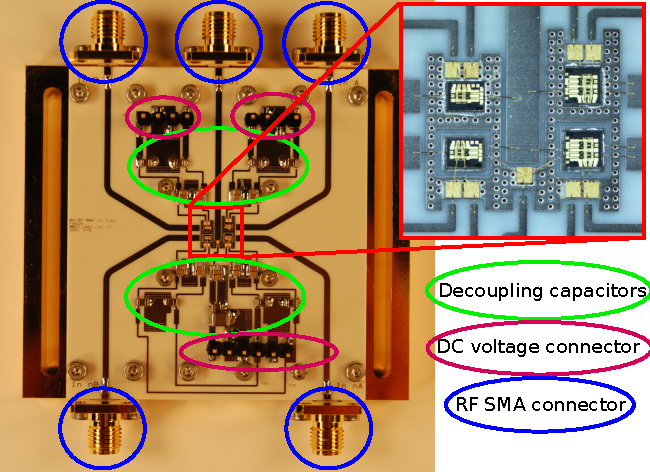
\includegraphics{Demonstrator_edited_newScale.pdf}
	\caption{Assembled demonstrator}
	\label{fig:assembledDemonstrator}
\end{figure}

\begin{figure}[htb!]
	\centering
  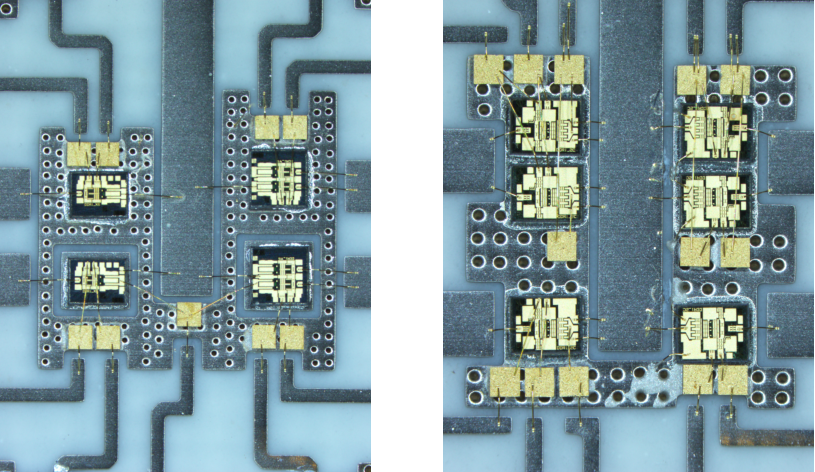
\includegraphics{ComparePhotoXY6_2C.pdf}
	\caption{Comparison of assembled chips DDRi\_X6 \& DDRi\_Y6 (left) and DDRi\_2C (right)}
	\label{fig:CompareChips}
\end{figure}

\newpage
Another approach would be to solder the DDRi\_XY6 chips on a electrical isolator while thermal (good) conductor as AluminiumNitrid (AlN: 180-200 W/mK -> datasheet). To ensure the isolation from output port to GND but still have a good thermal transfer.
This approach would have required only a small amount of the material AlN, which had to be cut very precisely into very tiny pieces.
This pads glued (adhesion, soldered) on the conduction layer for heat transfer. 
All in all this would be the better choice, but for the first proof of concept this would be more expensive.
In fact of the very small and precise size of the special material this would extend it.


\begin{figure}[htb!]
	\centering
  \includegraphics{Layout_DDRiXY6_AlN_pads.pdf}
	\caption{Improved layout for Chips DDRi\_X6 and DDRi\_Y6}
	\label{fig:DDRiXY6AlNpads}
\end{figure}
\chapter{Measurement}
\section{Measurement setup}
This section will describe the setup of the measurements. The approach was to resort to past designs and works of a former employee of IAF. Based on the work of Stephan Maroldt, i took some MMICs and Chips to get a first realisation of the work.
\begin{itemize}
	\item Keysight AWG - 1Vpp
	\item Broadband (35k-40GHz) amplifier (5Vpp out) (digital signal with clk 1GHz, 10 harmonics -> 10GHz)
	\item Bias Tee (DC bias)
	\item DC supply (driver network, power transistor)
	\item DUT (2x X6 + 2x Y6 Chip + filter network)
	\item LOAD - OUTPUT
\end{itemize}
Output measurement maybe with anteverta active load pull system. 
\section{Measurement results}
how to measure at the output of the schematic? is the measurement result as expected from the simulation?
\chapter{Conclusion-Outlook}
Problems, enhancement of the work, improvements, new design.

\nocite{Devrac2014}
\nocite{Devrac2015}


\cleardoublepage
\clearpage
\phantomsection

\addcontentsline{toc}{chapter}{\bibname}
\bibliographystyle{IEEEtran}
%\clearscrheadings
%\manualmark
%\markboth{Literature}{Literature}
\bibliography{literature}


%\renewcommand*\thechapter{}
\renewcommand*\thesection{\Alph{section}}
\chapter*{Appendix}
\chaptermark{Appendix}
\stepcounter{chapter}
\ifoot{Appendix}
\addcontentsline{toc}{chapter}{Appendix}

\section{Schematic of the Riemann Pump circuit}
bla bla bla bal bla lbal blalsl

\newpage
\section{Layout of the whole Riemann Pump circuit}

bla bla bla bal bla lbal blalsl

bla bla bla bal bla lbal blalsl

\newpage
\section{Photography of the realized Demonstrator}

bla bla bla bal bla lbal blalsl
%\cleardoublepage
%$\markboth{\nomname}{\nomname}
\cleardoublepage
%\Declaration

%\makeiheabstract

% Anhang/Appendix
%\begin{appendices}
%\renewcommand{\appendixtocname}{Anhang}
%\renewcommand{\appendixname}{Anhang}
%\addappheadtotoc
%\appendixpage
%\end{appendices}

\end{document}



	%\begin{tabular}{ll@{\hspace{1cm}}ll@{\hspace{1cm}}l}
